% Isto é um exemplo de Ficha Catalográfica, ou ``Dados internacionais de
% catalogação-na-publicação''. Você pode utilizar este modelo como referência. 
% Porém, provavelmente a biblioteca da sua universidade lhe fornecerá um PDF
% com a ficha catalográfica definitiva após a defesa do trabalho. Quando estiver
% com o documento, salve-o como PDF no diretório do seu projeto e substitua todo
% o conteúdo de implementação deste arquivo pelo comando abaixo:
%
\begin{fichacatalografica}
    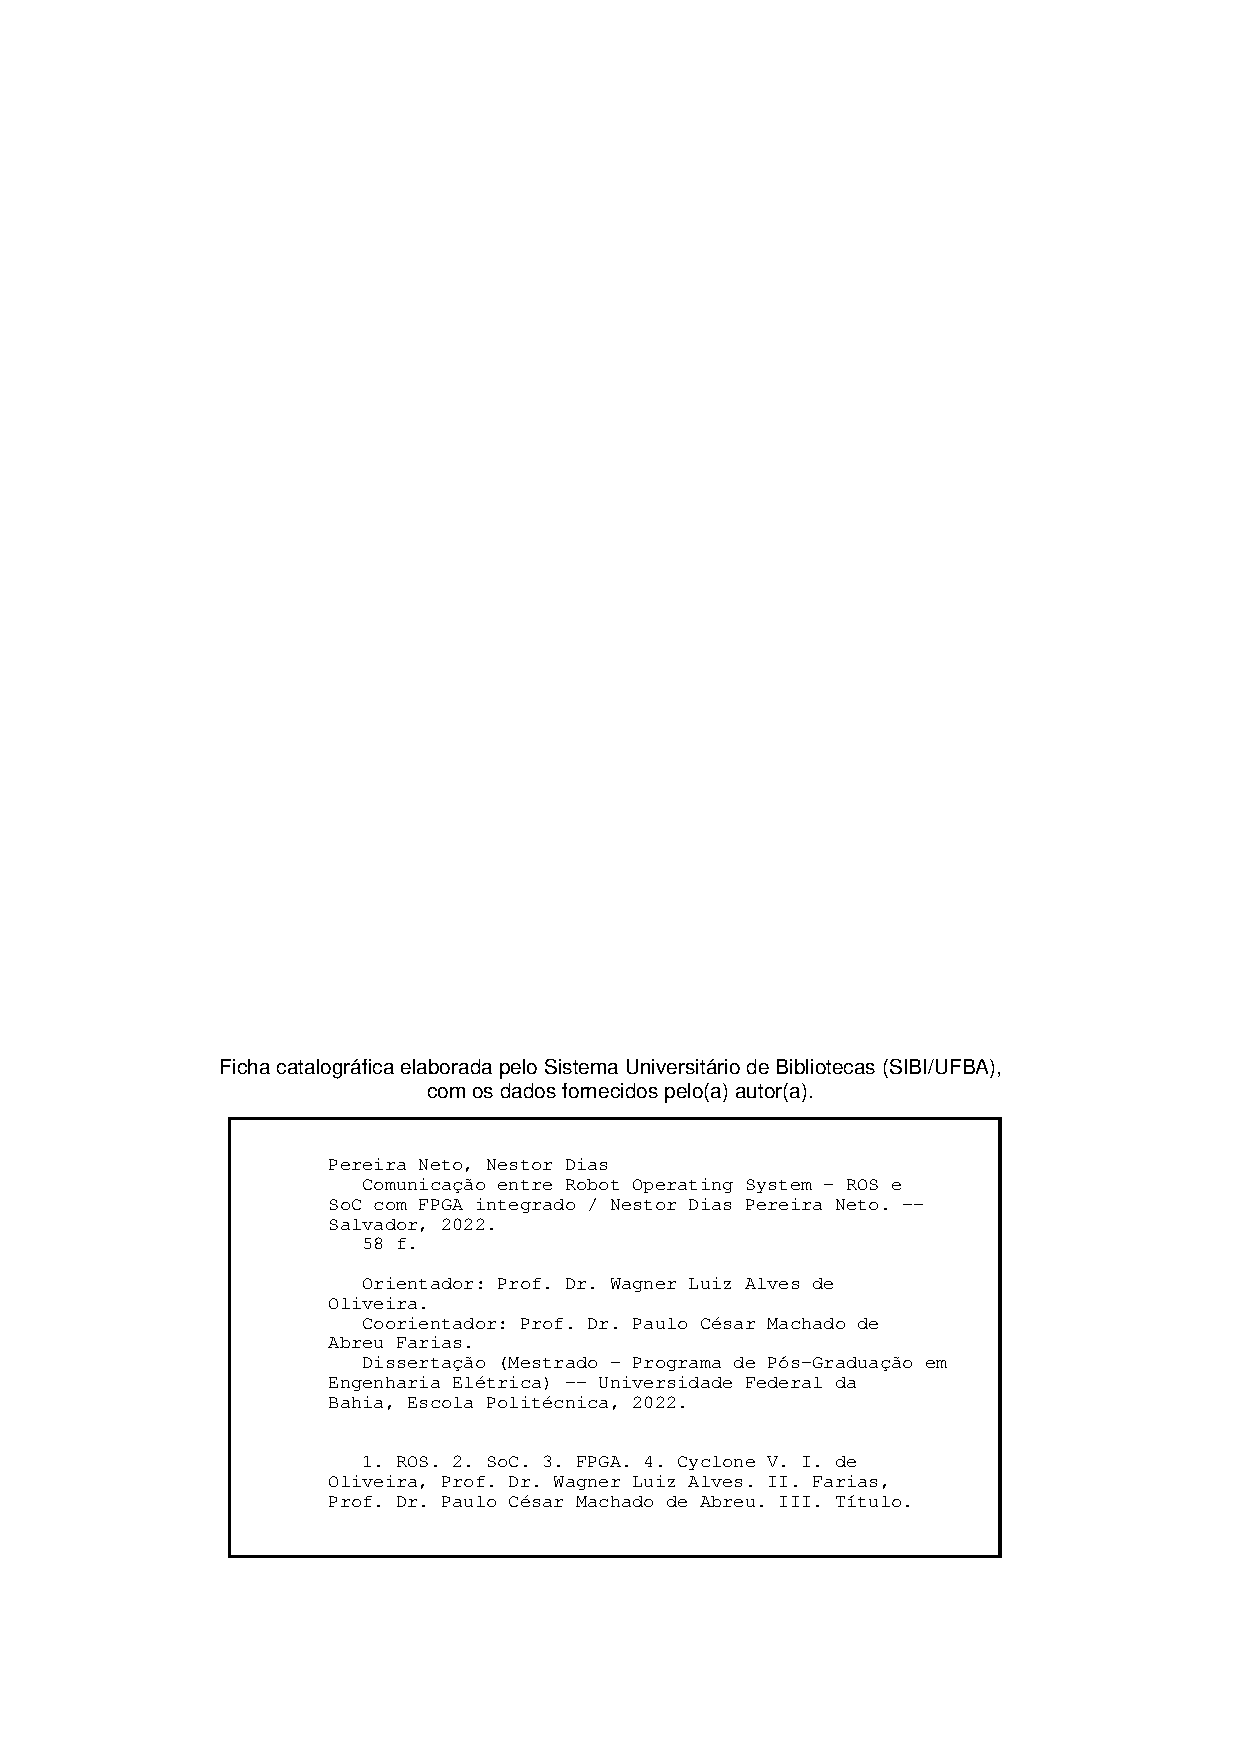
\includepdf{pre-textuais/ficha_dissertacao_nestor.pdf}
\end{fichacatalografica}
% \begin{fichacatalografica}
% 	\sffamily
% 	\vspace*{\fill}					% Posição vertical
% 	\begin{center}					% Minipage Centralizado
% 	\fbox{\begin{minipage}[c][8cm]{13.5cm}		% Largura
% 	\small
% 	\imprimirautor
% 	%Sobrenome, Nome do autor
	
% 	\hspace{0.5cm} \imprimirtitulo  / \imprimirautor. --
% 	\imprimirlocal, \imprimirdata-
	
% 	\hspace{0.5cm} \thelastpage p. : il. (algumas color.) ; 30 cm.\\
	
% 	\hspace{0.5cm} \imprimirorientadorRotulo~\imprimirorientador\\
	
% 	\hspace{0.5cm}
% 	\parbox[t]{\textwidth}{\imprimirtipotrabalho~--~\imprimirinstituicao,
% 	\imprimirdata.}\\
	
% 	\hspace{0.5cm}
% 		1. Palavra-chave1.
% 		2. Palavra-chave2.
% 		2. Palavra-chave3.
% 		I. Orientador.
% 		II. Universidade xxx.
% 		III. Faculdade de xxx.
% 		IV. Título 			
% 	\end{minipage}}
% 	\end{center}
% \end{fichacatalografica}
%---